\section{$X_{i}$を一つ前の$X_{j}$によって決まる確率で選び,その中から点$x$が一様に選ばれる場合}

次に考えるのは,$X_{i}$の選び方が,一つ前の$X$による確率で決定するような場合である。この確率を定めるにあたり,会議として自然と思われる$X_{i}$間に距離が定義でき,その距離にしたがって確率が決まるような問題を考えることとした。このとき距離の計算に用いることができるパラメータの数を$b$とし,距離として$b$次元ユークリッド距離を考えることにする。

すなわち$b$個のパラメータを要素とする元からなる空間$X$があったとき,
距離関数$d: X \times X \rightarrow \mathbb{R}$が
\[d(x, y) = \sqrt{\sum_{i=1}^{b}(x_{i}-y_{i})^{2}}\ \ ,\ x,y\in X\]
と書けることを意味する。実際の場合には,各データ同士の相関を考慮に入れたマハラノビス距離などのほうが適当な場合もあるかもしれないが,まずはイメージしやすいということでユークリッド距離を考えた。
以下では,記述を簡単にするため,$X_{i}$と$X_{j}$の間の距離を$d_{ij}$と書くことにする。

時刻$k$に$X_{i}$が選ばれ,その後時刻$k+1$に$X_{j}$から点$x_{k+1}^{j}$が選ばれる確率$p_{k}(i,j)$は,距離$d_{ij}$の関数として,次のようにできる。
\[p_{k}(i,j) = \frac{g_{k}(d_{ij})}{\sum_{j} g_{k}(d_{ij})}\]
ここでの関数$g$の選び方によって,距離の大きさがどのように確率に重みを持たせるかということが決定される。一般に$g$は時刻$k$によって変化してもいいので,添字$k$をつけて時刻$k$における関数であることを表した。

単純な例として$g_{k}(d) = const.,\ ^{\forall}k, d\in \mathbb{R}^{1}$とすると,距離に依らず$X_{i}$が選ばれるわけなので,3.1節の$X_{i}$の選び方と同じである。
$g(d)$は$[0, +\infty]$で定義される非負の実関数であればよい。

ex)
\[g(d) = \frac{1}{d+1}\]
\[g(d) = e^{-d}\]
\[g(d) = \left\{ \begin{array}{ll} c & (0\le d \le 1/c) \nonumber\\
1/d & (d>1/c)\end{array}\right., \ \ c>0\]

しかし,ここで注意すべき点として,どの$X_{i}$が選ばれたとしても,3.1で考えたように,どの$X_{i}$も$[0,1]$から一様に点$x$を取るから,結局点$x$について見たときの試行は同様のことをしており,どの$X_{i}$が選ばれるかは本質的な問題にはならないことが分かる。

これまでの設定を用いて数値シミュレーションを行った結果を図\ref{fig:f4}$\sim$\ref{fig:f6}に示す。シミュレーションでは,確率を決める距離の関数$g(d)$として
\[g(d) = e^{-d}\]
を採用し,$x$の次元$a=2$,$X_{i}$の数$N=6$と設定した。

図\ref{fig:f4}の中の青い丸が$X_{i}$の位置を表しており,それぞれの丸の大きさは,一回の試行において選択された頻度を表したものとなっている。円の間に張られた線分とそこに記された数字の組は,1番目の数字をラベルとしてもつ$X_{i}$のあとに2番目の数字をラベルとしてもつ$X_{j}$が選ばれたことを意味している。
図\ref{fig:f5}で青色の曲線で表されているのは,時刻$k$に選ばれた点$x$のまわりの$r$で決まる領域の中に入った,それまでに選択された点の数である。また,このグラフで緑色の直線として表されているものは,3.1のように計算で求めた値であり,
\[l = (-r^{2} + 2r)k\]
であった。このグラフを見て分かるように,理論値と実験値はよく一致していることが分かる。同じようにして偏差についても計算ができており,
$V(l) = \sqrt{(-r^{2} + 2r)(1+r^{2}-2r)k}$
である。これはグラフにおいて緑色の領域として描かれている。
図\ref{fig:f6}は,時刻$k$までに張られたエッジの数の総和を表しており,この中の緑色の曲線も,計算で求めることのできるものであった:
\[L = \frac{1}{2}(-r^{2} + 2r)k^{2}\]
この値もグラフから分かるように,よく理論値と一致していることが分かる。

\begin{figure}[H]
    \begin{center}
        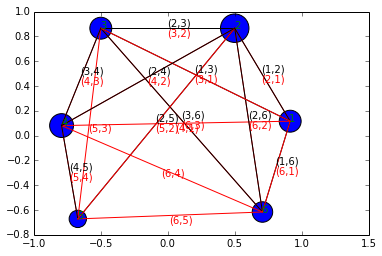
\includegraphics[width=10cm]{../download2_2.png}
        \caption{$X_{i}$の選択された頻度と$X_{i}$間ネットワーク}
        \label{fig:f4}
    \end{center}
\end{figure}
\begin{figure}[H]
    \begin{center}
        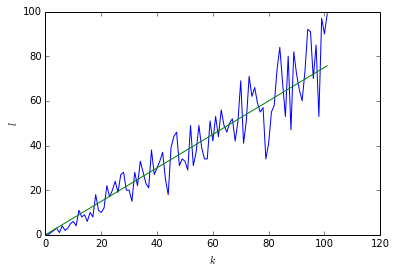
\includegraphics[width=10cm]{../download2_3.png}
        \caption{時刻$k$とその時張られたエッジの本数$l$との間の関係}
        \label{fig:f5}
    \end{center}
\end{figure}
\begin{figure}[H]
    \begin{center}
        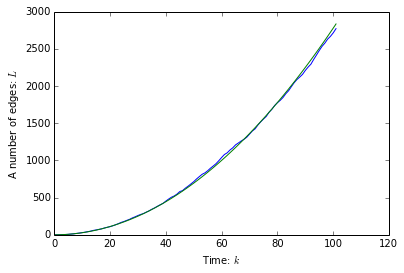
\includegraphics[width=10cm]{../download2_4.png}
        \caption{時刻$k$までに張られたエッジの数の総和$L$}
        \label{fig:f6}
    \end{center}
\end{figure}

また,図\ref{fig:f5}における直線の傾きは$r$に依存していたがこの傾きを$r$に関してプロットすると,以下の図\ref{fig:f7}のようになる。

\begin{figure}[H]
    \begin{center}
        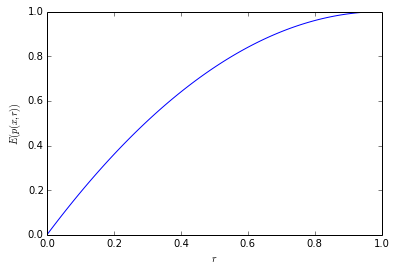
\includegraphics[width=10cm]{../download2_5.png}
        \caption{図\ref{fig:f5}の理論式直線の傾きと$r$の関係}
        \label{fig:f7}
    \end{center}
\end{figure}

図\ref{fig:f4}で,$r=1/3$としていたので,緑の直線の傾きは$-1/3(1/3-2) = 5/9$である。
